\documentclass[]{dithesis}
%\documentclass[suomi]{dithesis}


\usepackage{amsmath}
\usepackage{multirow}
\usepackage{array}

\title{Requirement and implementation specification and test plan}

\begin{document}

\maketitle

%%Document information
\paragraph{}
\begin{center}
\begin{tabular}{|p{4cm}|p{8cm}|}
\hline
\multicolumn{2}{|c|}{Document information} \\
\hline
Subject: & subject \\
\hline
\multirow{3}{4em}{Authors:} & Risto Korhonen \\
& Joakim Myllynen \\
& Vili-Jussi M\"akinen \\
\hline
Keywords: & Iot, Wireless sensor, Lte-M \\
\hline
Creation date: & 17 February 2023 \\
\hline
Revision date: & dd/mm/yyyy \\
\hline
Print date: & dd/mm/yyyy \\
\hline
\end{tabular}
\end{center}


%%Project information
\paragraph{}
\begin{center}
\begin{tabular}{|p{4cm}|p{8cm}|}
\hline
\multicolumn{2}{|c|}{Project information} \\
\hline
Course name: & Embedded System Project \\
\hline
Assistent: & Antti Tikanm\"aki \\
\hline
\multirow{3}{4em}{Document status:} & [x] Draft\\
& [ ] Proposal \\
& [ ] Inspected and accepted\\
\hline
\multirow{5}{4em}{Revision history:} & 1.0 Draft\\
& 1.1 \\
& 1.2 \\
& 1.3 \\
& 1.4 \\
\hline
\end{tabular}
\end{center}


%\abstractpage{Saarnisaari H. (2022) This is readme for \LaTeXe\ DI-thesis class.}{Faculty of Information Technology and Electrical Engineering, Degree Programme in Electronics and Communications Engineering, 10 pages.}{This document gives information that are required in order to finish the layout. The original direadme.tex-file provides also an example file of usage of the class. The direadme.ps-file gives an example of the final appearance}{\LaTeXe\, , dithesis}


\tableofcontents

%\prefacepage{This is my brief preface.\\ \\ Harri Saarnisaari}

\symbolspage{
\begin{tabular}{lll} 

ARM & \quad\quad & Advanced RISC Machine \\
BGA & \quad\quad & Ball Grid Array \\
e-INK & \quad\quad & Electronic Ink \\
ESD & \quad\quad & Electrostatic-sensitive Device \\
GND & \quad\quad & Ground line (negative supply) \\ 
GNSS & \quad\quad & Global Navigation Satellite System \\
GPIO & \quad\quad & General Purpose I/O  \\
GPS & \quad\quad & Global Positioning System \\
HTTPS & \quad\quad & Hypertext Transfer Protocol Secure \\
I2C & \quad\quad & Inter-Integrated Circuit \\
IoT & \quad\quad & Internet of Things \\ 
JTAG & \quad\quad & Joint Test Action Group \\
LED & \quad\quad & Light Emitting Diode \\
LTE-M & \quad\quad & Long-Term Evolution Machine Type Communication \\
MCU & \quad\quad & Microcontroller Unit \\
MQTT & \quad\quad & MQ Telemetry Transport \\
PCB & \quad\quad & Printed Circuit Board \\
SDK & \quad\quad & Software Development Kit \\
SIM & \quad\quad & Subscriber Identity Module \\
SMS & \quad\quad & Short Message Service \\
SPI & \quad\quad & Serial Peripheral Interface \\
SWD & \quad\quad & Serial Wire Debug \\
UART & \quad\quad & Universal Asynchronous Receiver Transmitter \\
Vcc & \quad\quad & Common-collector voltage (positive supply) \\

%$h$ &\quad\quad & a vector \\ 
%$f(x)$ & \\quad\quad & a function \\ 
\end{tabular} 
}

%%CHAPTER STARTS HERE
\chapter{Introduction}
\setcounter{page}{5} %use this to set page numbering correctly after the first chapter title
%\input{chapter text file}


\section{Purpose}

The purpose of this document is to specify what this device is about, what is wanted from it, and how it is
implemented and tested.

\textbf{Requirement specification} defines the requirements for the IoT sensor and preliminary measurements or actions which enable to define the implementation of the first version of the
device.

\textbf{Implementation specification} defines the implementation of IoT sensor and if required, tests that enable defining the implementation in sufficient detail. The implementation specification is based on the requirements of the requirement specification. Tt must give answers how each requirement becomes fulfilled. Implementation specification may contain several options for implementation. If possible, it would be good to estimate also the time required to complete each implementation.

\textbf{Test plan} defines the tests that are performed during and after the development process for the device. Tests must verify that the device meets the requirements.

\section{Scope}

Requirement specification covers the functional, physical and electrical requirements of the device.

Implementation specification covers the implementation techniques, protocols, components, PCB and
software.

Test plan covers descriptions of basic hardware, unit, integeration, system and regression tests.

\section{Human resources}

Project team includes Risto Korhonen, Vili-Jussi Mäkinen and Joakim Myllynen. The areas of responsibility are:

\begin{itemize}
    \item[] Electronics: Vili-Jussi Mäkinen, Joakim Myllynen
    \item[] Software: Risto Korhonen
    \item[] Integration: Vili-Jussi Mäkinen,
    \item[] Documentation: Joakim Myllynen
    \item[] HW testing: Vili-Jussi Mäkinen, Joakim Myllynen
    \item[] SW testing: Risto Korhonen
    \item[] Project management: All
\end{itemize}

\section{Overview}

The device will be an IoT sensor that has cellular connectivity and that operates with batteries. It measures at least temperature and humidity of the environment. It will send the measurements to the cloud over LTE-M or NB-IOT and show the measurements on the screen. One possible use case for the IoT sensor is to measure the temperature of a cottage and alert the user if the temperature goes bellow a set threshold. This way it is possible to prevent harmful events, ex. freezing the water pipes. Because the device is battery powered, it will continue to operate during an electrical break. 

\chapter{Requirement specification}

\section{Assumptions}

This prototype will be used by the developers only, so the ease-of-use is not highest priority. Further development of user interface and controls is needed if actual product is made.

\section{Functional requirements}

\begin{tabular}{| l | m{6.5cm} | m{6.5cm} |}
\hline
\textbf{Req No} & \textbf{Description} & \textbf{Parameters}  \\
\hline
Req 1.1 & Measure temperature and humidity & Update interval can be defined by user  \\
\hline
Req 1.2 & Show last measurement on display & Update interval can be defined by user  \\
\hline
Req 1.3 & Send last measurement to cloud & Update interval can be defined by user  \\
\hline
Req 1.4 & Alert user if temperature goes out of defined range & Temperature range  \\
\hline
Req 1.5 & Alert user if battery is running empty & \\
\hline
\end{tabular}

\section{User interface requirements}

\begin{tabular}{| l | m{6.5cm} | m{6.5cm} |}
\hline
\textbf{Req No} & \textbf{Description} & \textbf{Parameters}  \\
\hline
Req 2.1 & Display & 2.9" e-INK  \\
\hline
Req 2.1.1 & User can view measurement data &   \\
\hline
Req 2.1.2 & User can view battery status &  \\
\hline
Req 2.2 & User controls &  \\
\hline
Req 2.2.1 & Refresh button &  \\
\hline
Req 2.2.2 & Three buttons & Functionality to be determined \\
\hline
Req 2.3 & LEDs & \\
\hline
Req 2.3.1 & Green and red led & \\
\hline
\end{tabular}

\section{Connectivity requirements}

\begin{tabular}{| l | m{6.5cm} | m{6.5cm} |}
\hline
\textbf{Req No} & \textbf{Description} & \textbf{Parameters}  \\
\hline
Req 3.1 & SWD & Programming and debugging the device (JTAG equivalent from ARM) \\
\hline
Req 3.2 & LTE-M/NB-IoT & To send messages to cloud  \\
\hline
Req 3.2.1 & MQTT message/HTTPS request & Protocol to send messages to cloud  \\
\hline
Req 3.3 & GPS & To extend possible use cases \\
\hline
Req 3.4 & UART & Debugging and logging \\
\hline
\end{tabular}

\section{Electrical requirements}

\begin{tabular}{| l | m{6.5cm} | m{6.5cm} |}
\hline
\textbf{Req No} & \textbf{Description} & \textbf{Parameters}  \\
\hline
Req 4.1 & Must operate with 3x AA batteries &   \\
\hline
Req 4.1.1 & Internal operating voltage must be 3.3V & \\
\hline
Req 4.2 & Must have external sensor board & Board locates inside the device \\
\hline
Req 4.2.1 & Temperature sensor & TMP117 \\
\hline
Req 4.2.1 & Humidity sensor & HDC2010 \\
\hline
Req 4.3 & Device must have following antennas: & \\
\hline
Req 4.3.1 & LTE & \\
\hline
Req 4.3.2 & GPS & \\
\hline
Req 4.4 & Device must have a SIM card & \\
\hline
Req 4.4.1 & SIM-card holder & \\
\hline
Req 4.4.2 & SIM-card ESD protection & TPD3F303 \\
\hline
\end{tabular}

\section{Mechanical requirements}

\begin{tabular}{| l | m{6.5cm} | m{6.5cm} |}
\hline
\textbf{Req No} & \textbf{Description} & \textbf{Parameters}  \\
\hline
Req 5.1 & Casing &   \\
\hline
Req 5.1.1 & Made from plastic & \\
\hline
Req 5.1.2 & Must have space for 3 AA batteries & \\
\hline
Req 5.1.3 & Will be 3D-printed & \\
\hline
\end{tabular}

\section{Other requirements}

\begin{tabular}{| l | m{6.5cm} | m{6.5cm} |}
\hline
\textbf{Req No} & \textbf{Description} & \textbf{Parameters}  \\
\hline
Req 6.1 & Operating time & More than 6 months  \\
\hline
Req 6.2 & Operating conditions & \\
\hline
Req 6.2.1 & Operating temperature & -40C - 40C \\
\hline
Req 6.2.2 & Operating humidity & Normal room humidity \\
\hline
\end{tabular}

\chapter{Implementation specification}

\section{Hardware}

\subsection{Block diagram}

\begin{figure}[hbt!]
    \centering
    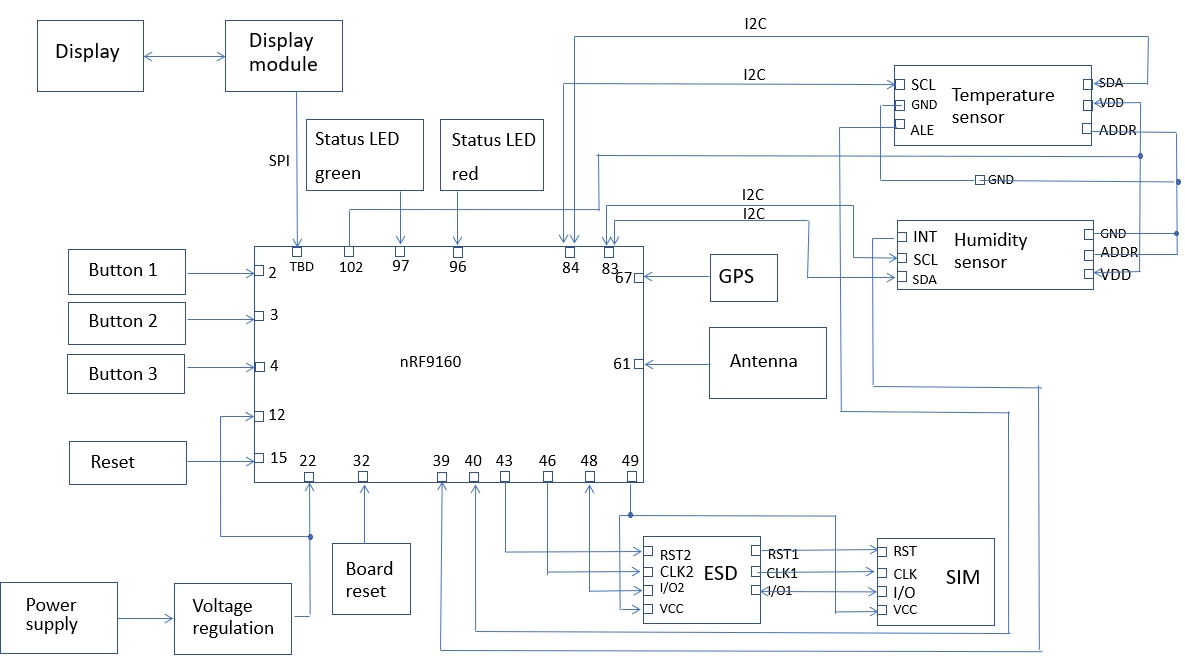
\includegraphics[width=16cm]{blockdiagramsulari.png}
    \caption{Block diagram and early schematic of the device.}
    \label{fig:my_label}
\end{figure}

\subsection{MCU selection}

For this project Nordic Semicoductor nRF9160 SIP was chosen. nRF9160 is a complete solution that includes application processor, multimode LTE-M/NB-IoT/GNSS modem, RF front end and power management IC in a single package. This simplifies the development as Nordic has good libraries for managing the modem from application code. Nordic also provides nRF SDK with Zephyr OS that includes drives for peripherals (I2C, modem, timers etc). C programming language will be used to program the processor.  

Dedicated application processor is 64MHz Arm Cortex-M33 with 1MB flash and 256KB of RAM. This should be enough, as the purpose is to take measurements and send them to the cloud instead of storing them in the device. Only the last measurement will be saved and show at the screen. 

nRF9160 can be operated with various input voltages form 1.8V to 5.5V. 

\begin{figure}[hbt!]
    \centering
    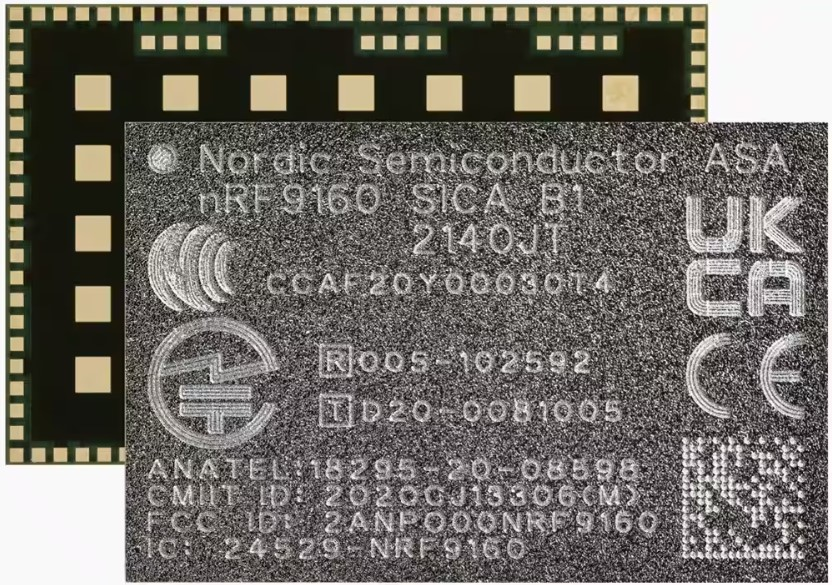
\includegraphics[width=5cm]{nRF9160.jpg}
    \caption{nRF9160 SiP.}
    \label{fig:my_label}
\end{figure}

\newpage

\subsection{Sensors}

Temperature sensor TMP117 and humidity sensor HDC2010 will be used.  An external board will be designed for the sensors. This way the sensors can be moved further from MCU and components that could warm up and thus affect the measurements. Power, I2C signals and possible interrupt signals are transferred between the sensor board and MCU. 

TMP117 is used for measuring temperature. It is chosen because of it's precision and connectivity, as it uses I2C bus to connect to the MCU. This makes connecting it to the MCU easy. It also has alert signals that can be configured to inform MCU if the temperature is outside of a specified range. This adds many interesting use cases, as well be discussed later in the document. HDC2010 will be used for measuring humidity, and the same selection principles are used as 

\subsection{Display}

WaveShare e-INK display module is used to display the last measurement and battery status. e-INK screen is chosen because it consumes power only when the screen is refreshed, so it reduces the power consumption of the device. Size of the module is 2.9” and resolution is 296 x 128 pixels. Screen has two colors, black and white. Screen module uses SPI to communicate with MCU.  

\subsection{Antennas}

Antennas for cellular and GNSS (GPS) are required. Purpose is to use already available antenna modules. PCB antennas could be an option, but it would require lots of designing and time and would add some uncertainty for the project, because none in the team has any experience about designing a PCB antenna. 

A Molex 2133530200 combo antenna for LTE and GPS is selected, mainly because of relatively good looking specs and cheap price. It also makes the assemby less complicated because there is less parts.

\subsection{Buttons}

4 buttons will be used to interact with user. Buttons will be connected to nRF9160 GPIO pins with proper pull-up or pull-down resistors. 

\subsection{LEDs}

2 leds will be used to inform the user. Red and green led will be connected to nRF9160 GPIO pins. Leds will inform the user in a way that will be determined (possible status indication and debugging information). Leds will be connected directly to the PCB, so they will not be visible outside of the device. 

\subsection{Power}

Three AAA batteries will be used to power the device. A voltage regulator will be used, but the exact model and circuitry will be determined. The device itself requires operating voltage of 3.3V. 

MCU current in different situations (3.7V):
\begin{itemize}
    \item System disabled: 150 nA 
    \item CPU
    \begin{itemize}
        \item Idle: 1 – 18 uA (depending on sleep mode)
        \item Active: 2.2 mA 
    \end{itemize}
    \item Cellular modem transmitting: 45 – 115 mA 
    \item GPS 
    \begin{itemize}
        \item Continuous tracking: 44.3 mA  
        \item Power saving mode: 9.6 mA 
    \end{itemize}
    \item Approximately 0.5 mA per system peripheral 
\end{itemize}

Other peripherals: 
\begin{itemize}
    \item Display: https://www.overleaf.com/project/63ef5776001f962c73785802
    \begin{itemize}
        \item Refresh: 5mA
        \item Standby: 10nA
    \end{itemize}
    \item Temperature sensor: 3.5 uA 
\end{itemize}


\section{Software}

\subsection{Software architecture}

nRF SDK is used for the main platform for the software. nRF SDK provides Zephyr OS that is customed to nRF9160. SDK provides essential drivers for the peripherals (SPI, I2C, GPIO...) and a complete LTE stack as well as application layer protocols such as HTTPS and MQTT.  

Most of the software can be done within the nRF SDK. What needs to be done is write/import a couple of drivers for environment sensors and the e-INK display as there is not ready-made drivers for nRF9160. These drivers will be implemented similarly to drivers provided by nRF SDK. 

\subsection{Flow diagram}

\begin{figure}[hbt!]
    \centering
    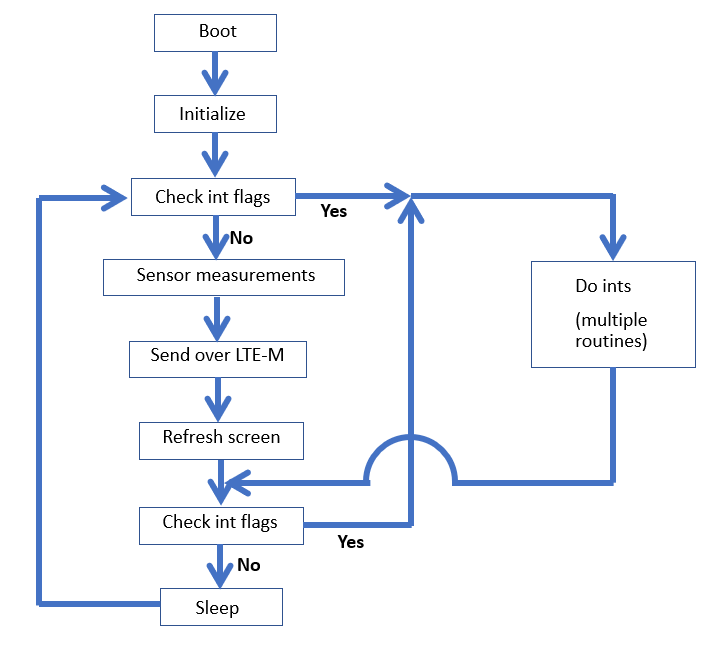
\includegraphics[width=12cm]{flowdiagram_sulari.png}
    \caption{Flow diagram of the main loop.}
    \label{fig:my_label}
\end{figure}


\subsection{Initialization and main loop}

During the boot software, OS and peripherals are initialized to known state.  

Main loop will be as shown in the figure (to be done). First the sensors are read through an I2C bus. After that the values are sent to the cloud and the display will be refreshed. Then the processor will be put to sleep for time that is defined by the user (typically something between 30s to 10min to obtain better battery life). 

\subsection{Interrupts}

Interrupts will be used for reacting to four buttons and responding to TMP117 alert signal and HDC2010 interrupt signal.

\subsection{Sensors}

The drivers for sensors must be imported/written. As the sensors use the I2C bus, the I2C driver is delivered to the sensor's driver through parameter so that the driver is not bounded to one specific I2C driver and is as re-usable as it can be. Maybe function pointers are used to initialize the I2C write/read functions to the sensor drivers. 

\subsection{e-INK screen}

The driver for e-INK screen must be imported. The screen uses SPI bus, so the existing SPI driver from nRF SDK will be used.

\subsection{Temperature out-of-range alert}

TMP117 temperature sensor has an option that it can trigger an external ALERT-pin if the measured temperature exceeds the user defined limits. ALERT-pin will be connected to one of the nRF9160 GPIO pins and that pins interrupt will be enabled. If the ALERT pin is triggered, the software will perform a routine that sends an immediate message to user instead of waiting for the defined refresh time. The message might be possible to send as SMS to user phone for higher noticeability, but that will be defined later. 

\section{Cost calculations}

Already bought items:
\begin{itemize}
    \item nRF9160 DK (borrowed from Nordic Semiconductor)
    \item TMP117 module 13.15€ (for breadboard prototyping)
    \item WaveShare e-INK module 2,9" 21.13€ (postage 5,90€)
    \item Things Mobile IoT SIM, 3pcs, 5€/pcs, postage 10€
\end{itemize}

\bigskip

Items to be bought:
\begin{itemize}
    \item TMP117 5€
    \item HDC2010 4€
    \item Antenna module 2,70€
    \item GPS Antenna module 4€
    \item LEDs < 1€
    \item Buttons approximately 2€
    \item Battery holder < 1€
    \item PCB approximately 20€
    \item ESD TPD3F303 < 1€
    \item Small general components 15€
    \item Casing (free)

\end{itemize}
\bigskip
Sum: Approximately 81e (+ postages) per device

\section{Tools}

Nordic semiconductor nRF9160 DK development kit is used to prototype and write software in the early phases when the application specific hardware isn't completed yet. Example sensor and screen drivers can be developed and tested independently from target hardware. It also provides a reference when testing the real hardware. Development kit can also be used to program the traget device and use as a debugger so no external programmer is needed.

KiCad 7.0 will be used to draw the schematics and desing the layout. Visual Studio Code with nRF SDK addon will be used to develop the software. 

The board will be soldered using the soldering oven in FabLab, as the nRF9160's footprint is BGA. Also FabLab's oscilloscope, power supply, multimeter, microscope and soldering stations will be used. 

\chapter{Testing}
\section{Hardware tests}

\subsection{Board assembled, power off}

\begin{tabular}{| m{2cm} | m{10cm} | m{2.5cm} |}
\hline
\textbf{Req No} & \textbf{Description} & \textbf{Result}  \\
\hline
Test 1.1.1 & No shortcuts or bad solder connections shown in visual \newline inspection &  \\
\hline
Test 1.1.2 & GND and Vcc lines are not shortcutted &   \\
\hline
Test 1.1.3 & GND is in contact from DC connector to the GND pins of IC &  \\
\hline
Test 1.1.4 & Vcc line is in contact from DC connector to the Vcc pins of IC & \\
\hline
Test 1.1.5 & GND and Vcc of the sensor board are in contact with GND and Vcc nets of the PCB & \\
\hline
Test 1.1.6 & Data pins of the sensor board are in contact with \newline corresponding pins in MCU & \\
\hline
Test 1.1.7 & Data pins of the sensor board are not connected to GND or VCC & \\
\hline
Test 1.1.8 & Lte antenna is connected to Lte antenna pin in the MCU & \\
\hline
Test 1.1.9 & GNSS antenna is connected to GNSS antenna pin in the MCU & \\
\hline
Test 1.1.10 & Reset button is connected to reset pin in the MCU & \\
\hline
Test 1.1.11 & Buttons 1, 2, 3 and 4 are connected to corresponding GPIO pins in the MCU & \\
\hline
Test 1.1.12 & All the buttons have proper pull-up or pull-down resistors in series with them & \\
\hline
Test 1.1.13 & All the leds have proper resistors connected in series with them & \\
\hline
Test 1.1.14 & GND and Vcc of the display module are connected to GND and Vcc nets of the PCB & \\
\hline
Test 1.1.15 & Data pins of the display module are connected to \newline corresponding pins in the MCU & \\
\hline
Test 1.1.16 & & \\
\hline
\end{tabular}

\subsection{Board assembled, power on}

\begin{tabular}{| m{2cm} | m{10cm} | m{2.5cm} |}
\hline
\textbf{Req No} & \textbf{Description} & \textbf{Result}  \\
\hline
Test 1.2.1 & Devices power consumption is under 50mA &  \\
\hline
Test 1.2.2 & Voltage between Vcc and GND is 3.3V within tolerance of 0.2V &   \\
\hline
Test 1.2.3 & Any component doesn't heat up rapidly &  \\
\hline
Test 1.2.4 & Vcc is measured in places where Vcc should be (SiP Vcc pin, sensor board Vcc connections, display module vcc connector) & \\
\hline
Test 1.2.5 & & \\
\hline
\end{tabular}

\section{Unit tests}

\begin{tabular}{| m{3cm} | m{12cm} | }
\hline
\textbf{Test 2.1} & \textbf{nRF9160 is booting up}  \\
\hline
Tools & Assembled device board   \\
\hline
Steps & Power on the board  \\
\hline
Accepted result & MCU boots up \\
\hline
Test result & \\
\hline
\end{tabular}

\bigskip

\begin{tabular}{| m{3cm} | m{12cm} | }
\hline
\textbf{Test 2.2} & \textbf{Sensor board is operational}  \\
\hline
Tools & Assembled device board and assembled sensor board, connector cable   \\
\hline
Steps & Connect sensor board to device board. Power on the board. Flash sensor test to the board.\\
\hline
Accepted result & MCU reads values from sensors \\
\hline
Test result & \\
\hline
\end{tabular}

\bigskip

\begin{tabular}{ | m{3cm} | m{12cm} | }
\hline
\textbf{Test 2.2.1} & \textbf{Temperature sensor accuracy sufficient}  \\
\hline
Tools & Assembled device board, sensor board, external temperature meter \\
\hline
Steps & Measure temperature with sensor and temperature meter, repeat measures 10 times and mark the results, calculate average values, compare values\\
\hline
Accepted result & Results from sensor and temperature meter are within 0.2 degrees celcius. \\
\hline
Test result & \\
\hline
\end{tabular}

\bigskip

\begin{tabular}{ | m{3cm} | m{12cm} | }
\hline
\textbf{Test 2.2.2} & \textbf{Humidity sensor accuracy sufficient}  \\
\hline
Tools & Assembled device board, sensor board, external humidity meter \\
\hline
Steps & Measure humidity with sensor and humidity meter, repeat measures 10 times and mark the results, calculate average values, compare values \\
\hline
Accepted result & Results from sensor and humidity meter are within 2 percentage point. \\
\hline
Test result & \\
\hline
\end{tabular}

\bigskip

\begin{tabular}{| m{3cm} | m{12cm} | }
\hline
\textbf{Test 2.3} & \textbf{Screen is operational}  \\
\hline
Tools & Assembled device board and screen module, connector cable   \\
\hline
Steps & Connect screen module to device board. Power on the board. Flash board test to the board.\\
\hline
Accepted result & Screen shows the content determined in screen test \\
\hline
Test result & \\
\hline
\end{tabular}

\bigskip

\begin{tabular}{| m{3cm} | m{12cm} | }
\hline
\textbf{Test 2.4} & \textbf{LTE-M is operational}  \\
\hline
Tools & Assembled device board, LTE antenna module, SIM card  \\
\hline
Steps & Connect LTE antenna and sim card to the device board. Power on the board. Flash LTE test to the board.\\
\hline
Accepted result & MCU sents a test message to MQTT broker/HTTPS endpoint. \\
\hline
Test result & \\
\hline
\end{tabular}

\bigskip

\begin{tabular}{| m{3cm} | m{12cm} | }
\hline
\textbf{Test 2.5} & \textbf{GPS is operational}  \\
\hline
Tools & Assembled device board, GPS antenna \\
\hline
Steps & Connect GPS antenna to the device board. Power on the board. Flash GPS test to the board.\\
\hline
Accepted result & MCU prints GPS coordinates to terminal. \\
\hline
Test result & \\
\hline
\end{tabular}

\iffalse

%%APPENDIX
\chapter{APPENDICES} %ENGLISH TITLE
Appendix 1 \quad A proof \\
Appendix 2 \quad Another proof

%\chapter{LIITELUETTELO} %FINNISH TITLE
%Liite 1 \quad A proof \\
%Liite 2 2 \quad Another proof

\newpage
\noindent Appendix 1 \quad A proof\\ \\
Appendices could contain mathematical proofs or computer program listings that are too lengthy for the main text.

\newpage
\noindent Appendix 2 \quad Another proof\\ \\
It is shown that $1=1$.

\fi

\end{document}







